\chapter{Additional comparisons with theoretical predictions}\label{app:NLO}

The cross section results for combined channel in fiducial regions have been compared to NNLO predictions for different PDF sets in Sec.~\ref{sec:CombCs}. This appendix presents the comparison of cross section in full and extrapolated to 13 TeV regions with NNLO predictions (Fig.~\ref{fig:AppD1}-Fig.~\ref{fig:AppD3}). The agreement between predictions and results in full region is worse, than for fiducial and extrapolated regions, however it is still within 2$\sigma$ of uncertainty. 

Additionally, the comparison for NLO predictions in fiducial region is presented in Fig.~\ref{fig:AppD4}-~\ref{fig:AppD5}.

\begin{figure}[!h]
\begin{minipage}[h]{0.49\linewidth}
\center{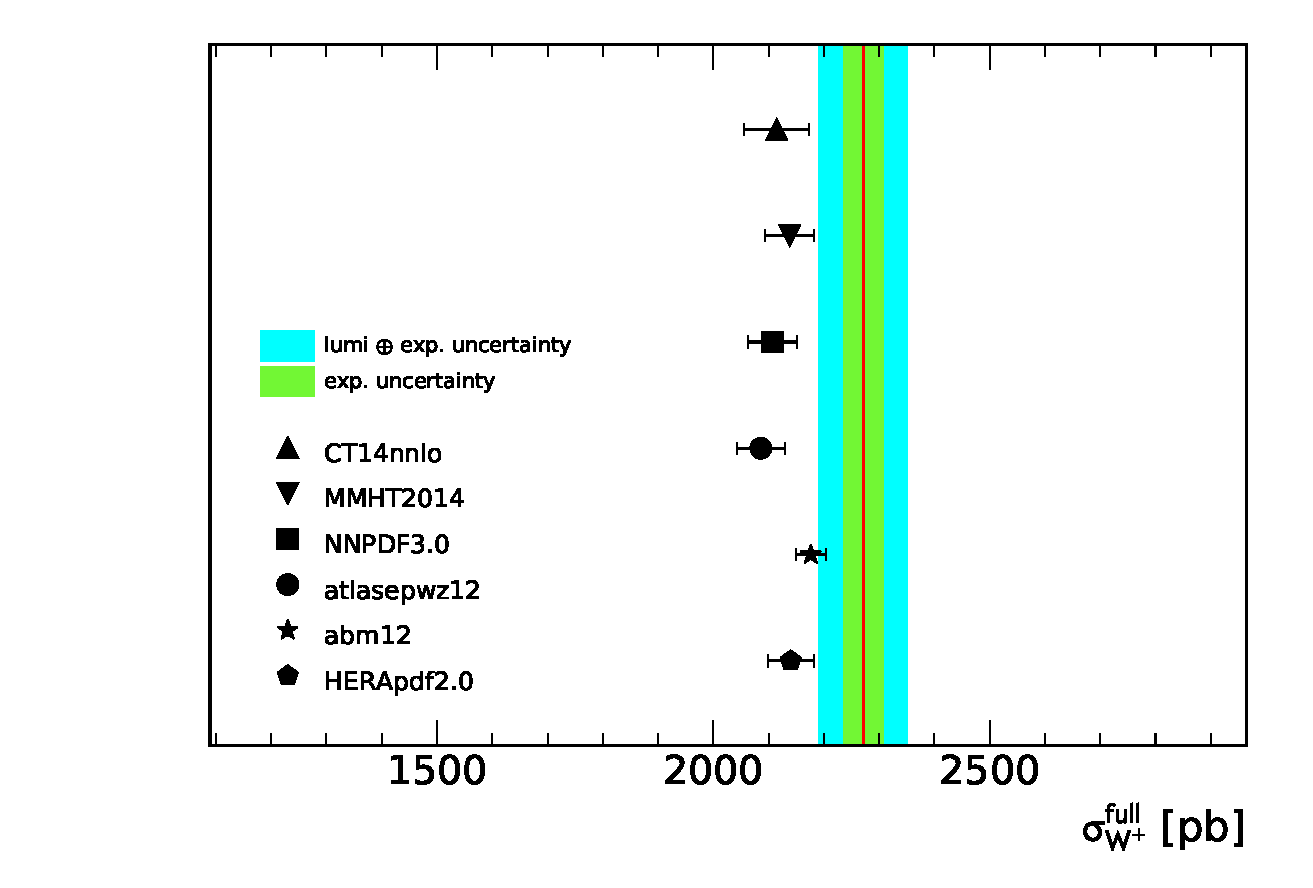
\includegraphics[width=1\textwidth]{Results/NNLOWpfull.pdf} \\ a)}
\end{minipage}
\hfill
\begin{minipage}[h]{0.49\linewidth}
\center{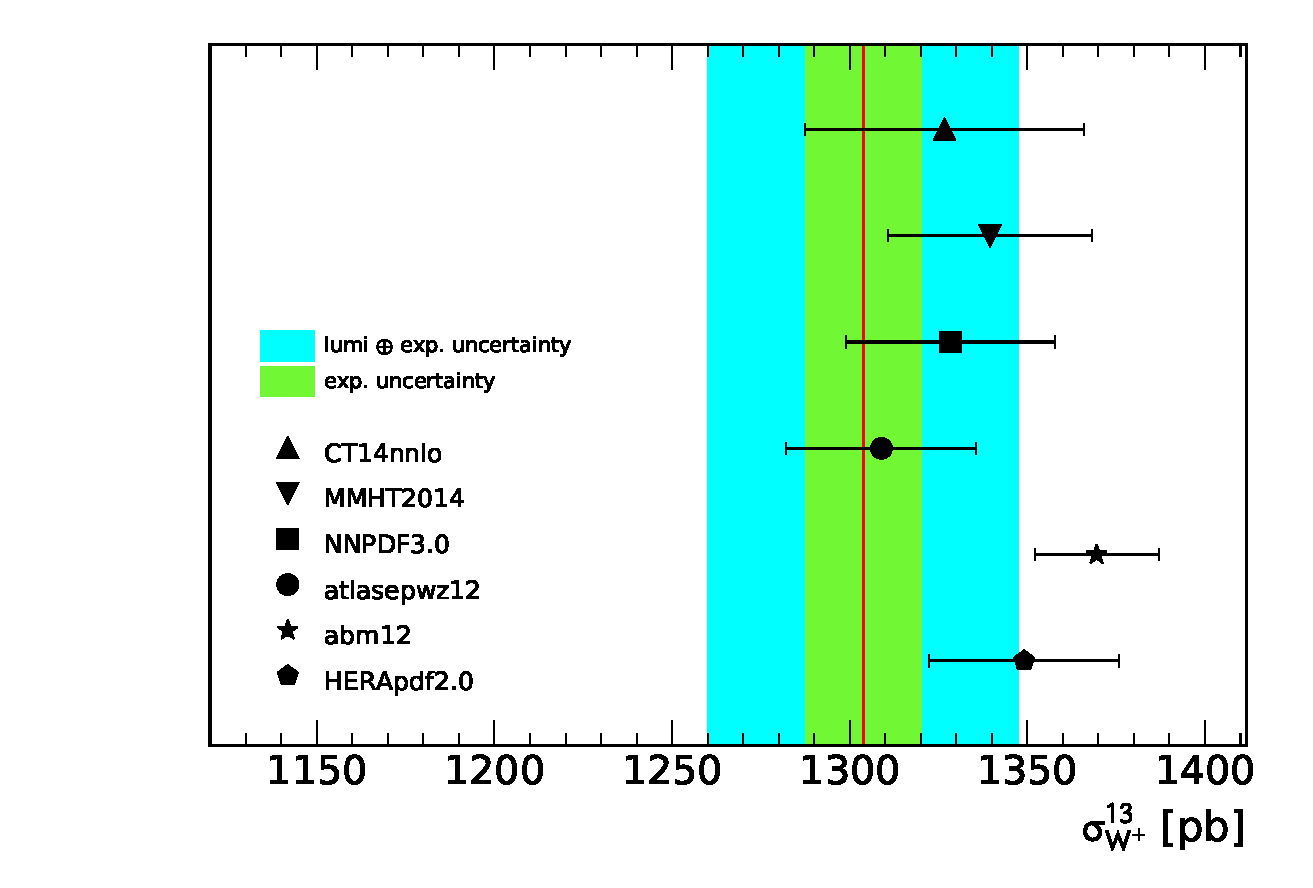
\includegraphics[width=1\textwidth]{Results/NNLOWp13.pdf} \\ b)}
\end{minipage}
\caption{The NNLO predictions for the $W^{+}$ cross section in a) full phase space and  b) new 13 TeV phase space in pb for the six PDFs CT14nnlo, MMHT2014, NNPDF3.0, ATLASepWZ12, abm12, HERApdf2.0 compared to the measured cross section as given in Tab.~\ref{tab:csComb}. The green (cyan) band corresponds to the experimental uncertainty without (with) the luminosity uncertainty. The theory predictions are given with the corresponding PDF uncertainties shown as error bands.}
\label{fig:AppD1}
\end{figure}


\begin{figure}[!h]
\begin{minipage}[h]{0.49\linewidth}
\center{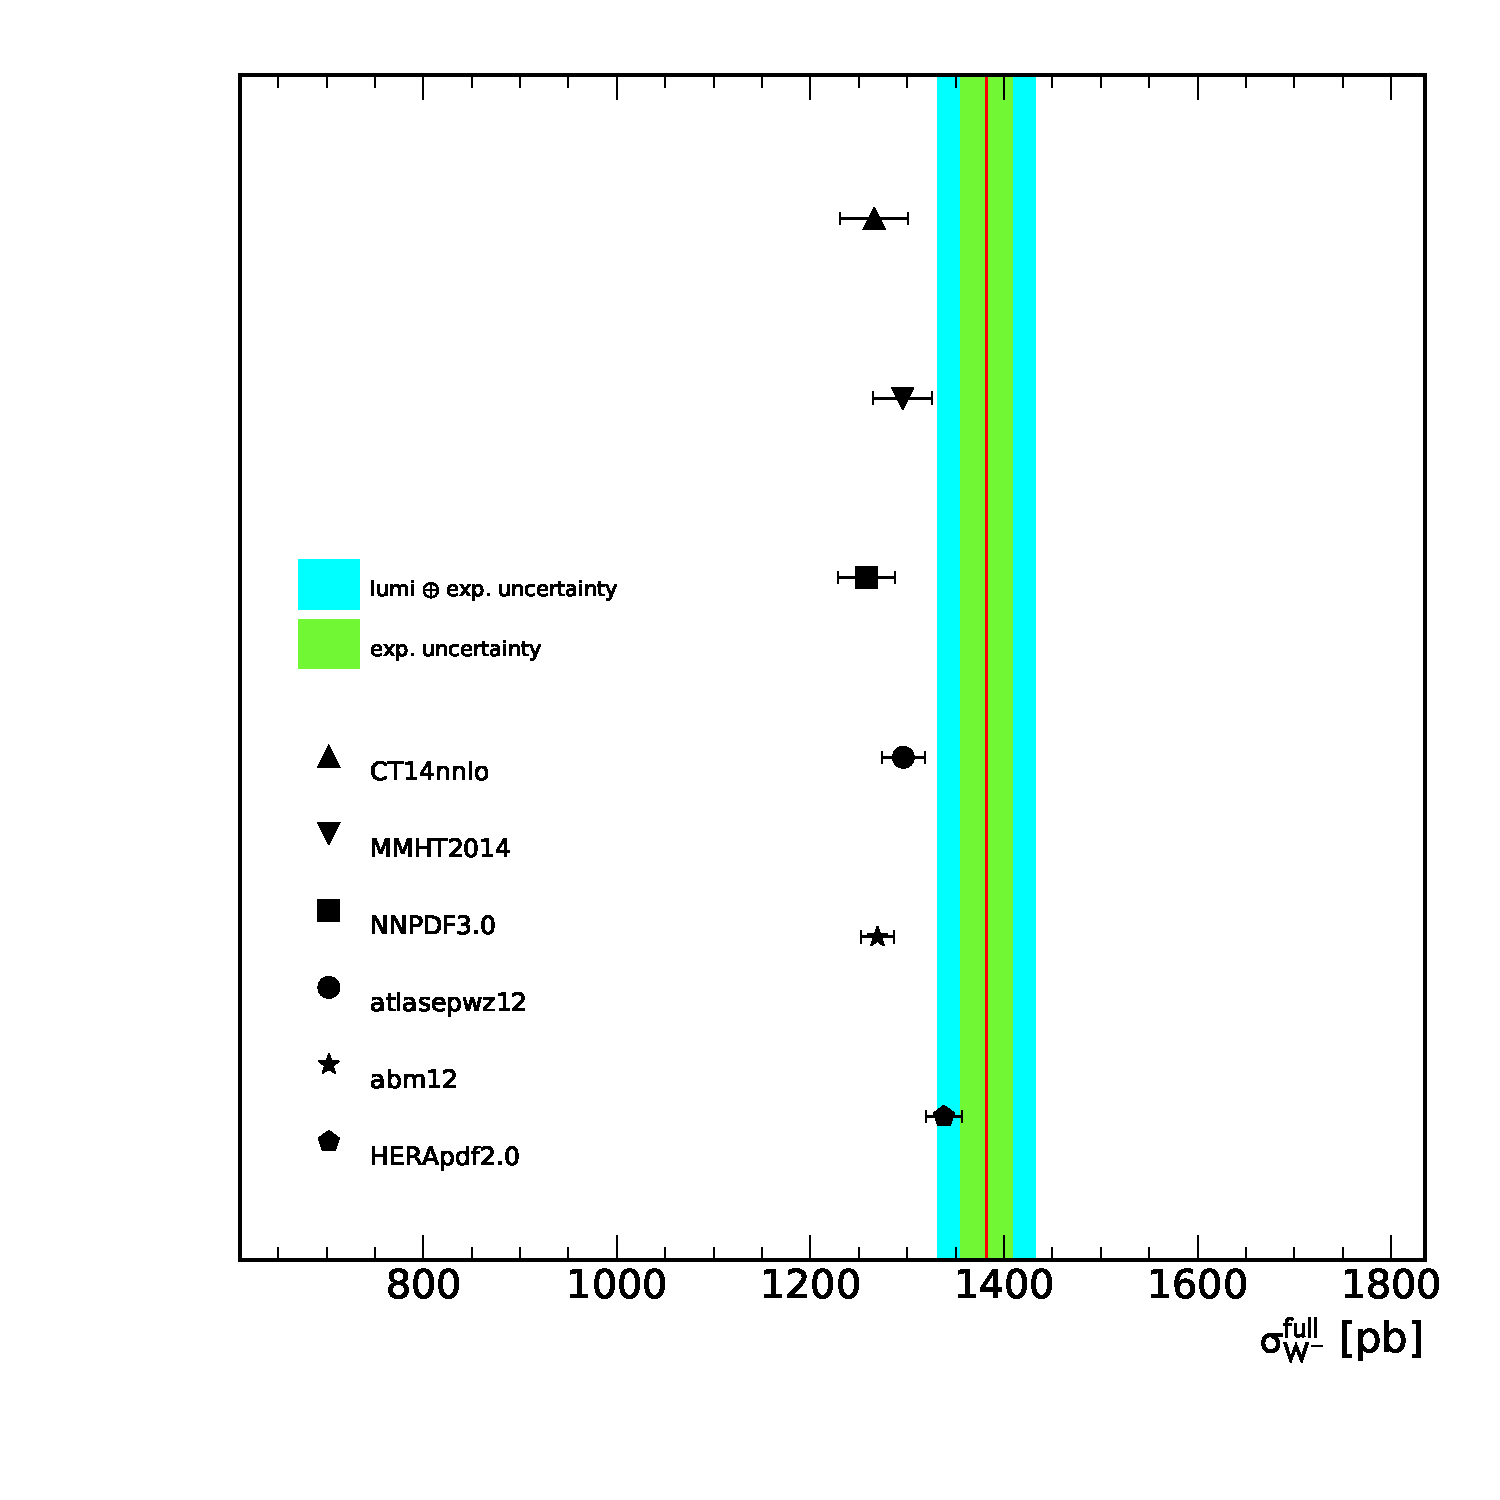
\includegraphics[width=1\textwidth]{Results/NNLOWmfull.pdf} \\ a)}
\end{minipage}
\hfill
\begin{minipage}[h]{0.49\linewidth}
\center{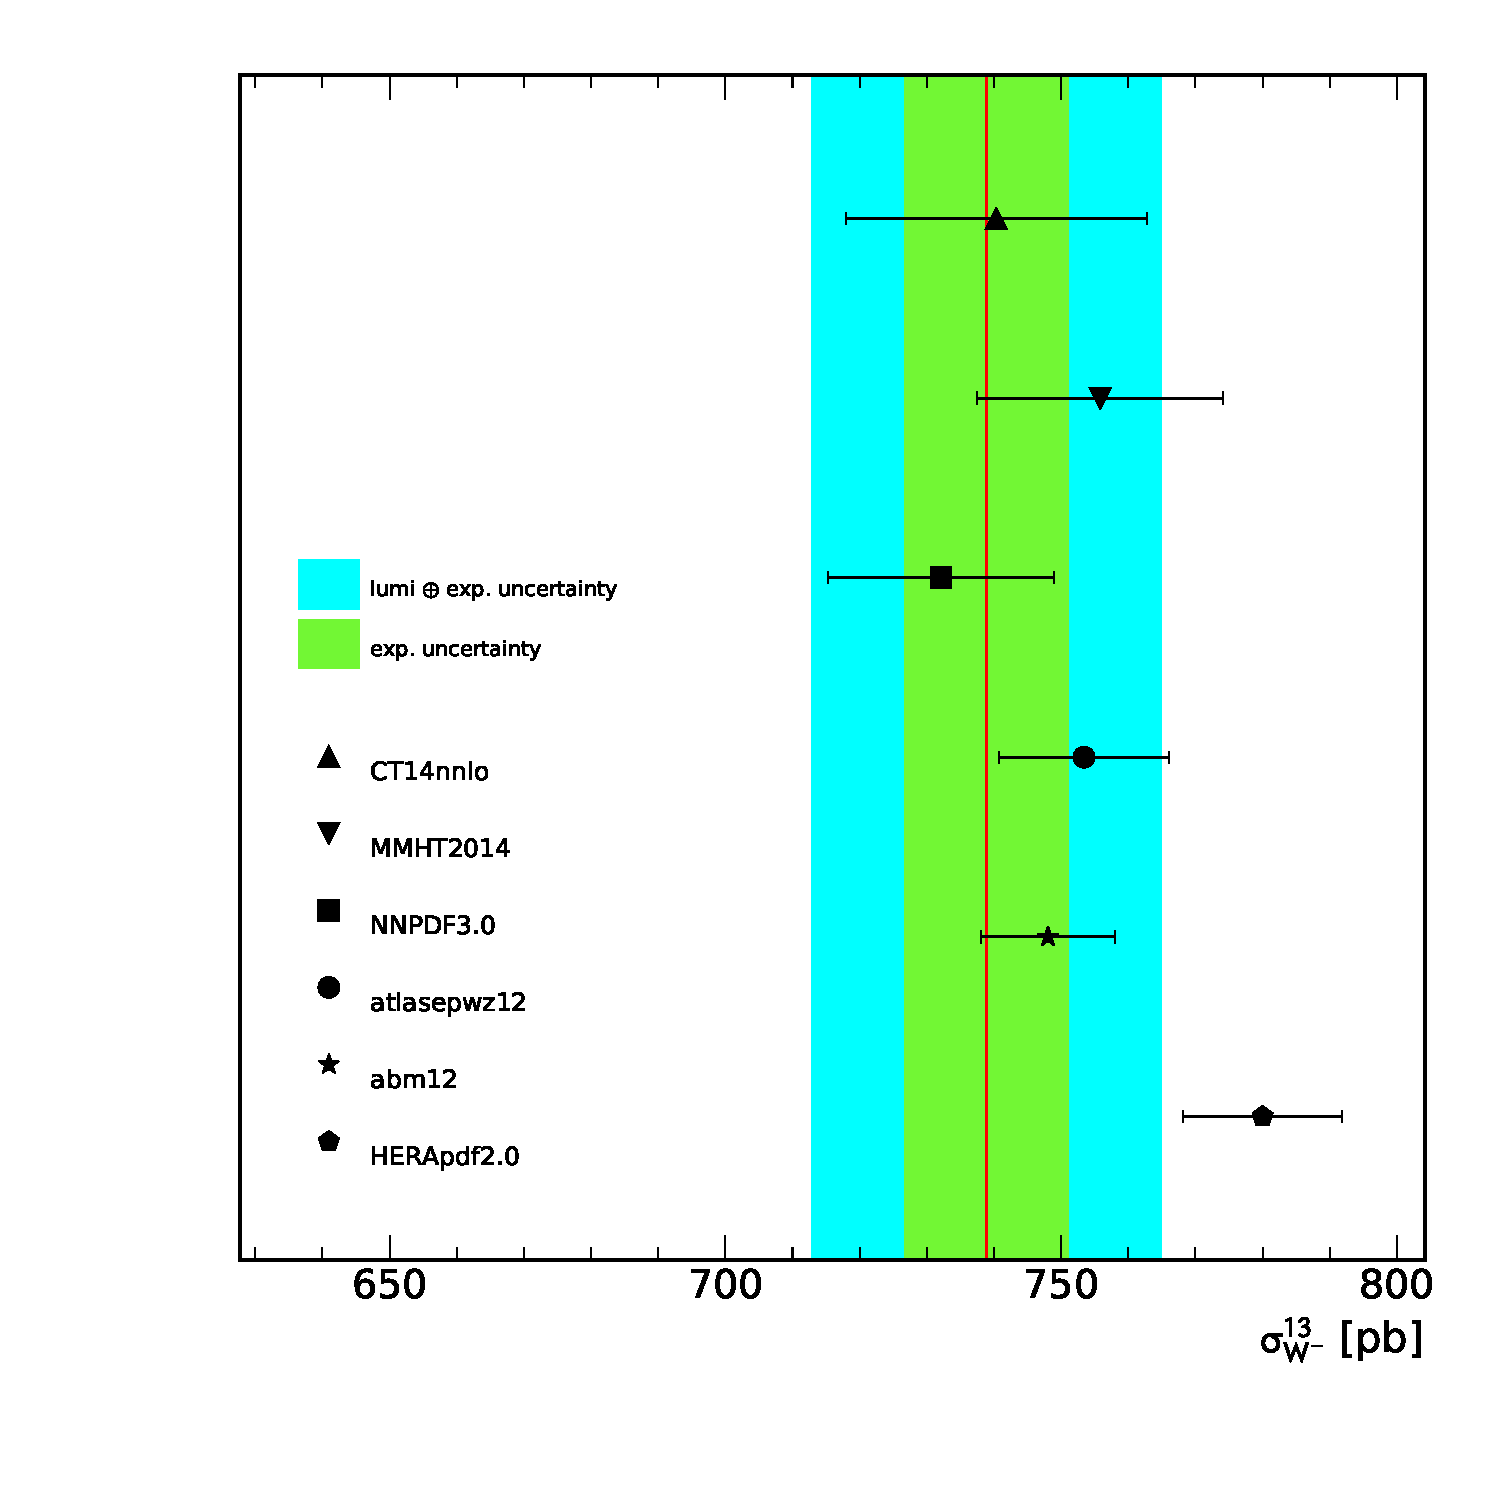
\includegraphics[width=1\textwidth]{Results/NNLOWm13.pdf} \\ b)}
\end{minipage}
\caption{The NNLO predictions for the $W^{-}$ cross section in a) full phase space and  b) new 13 TeV phase space in pb for the six PDFs CT14nnlo, MMHT2014, NNPDF3.0, ATLASepWZ12, abm12, HERApdf2.0 compared to the measured cross section as given in Tab.~\ref{tab:csComb}. The green (cyan) band corresponds to the experimental uncertainty without (with) the luminosity uncertainty. The theory predictions are given with the corresponding PDF uncertainties shown as error bands.}
\label{fig:AppD2}
\end{figure}

\begin{figure}[!h]
\begin{minipage}[h]{0.49\linewidth}
\center{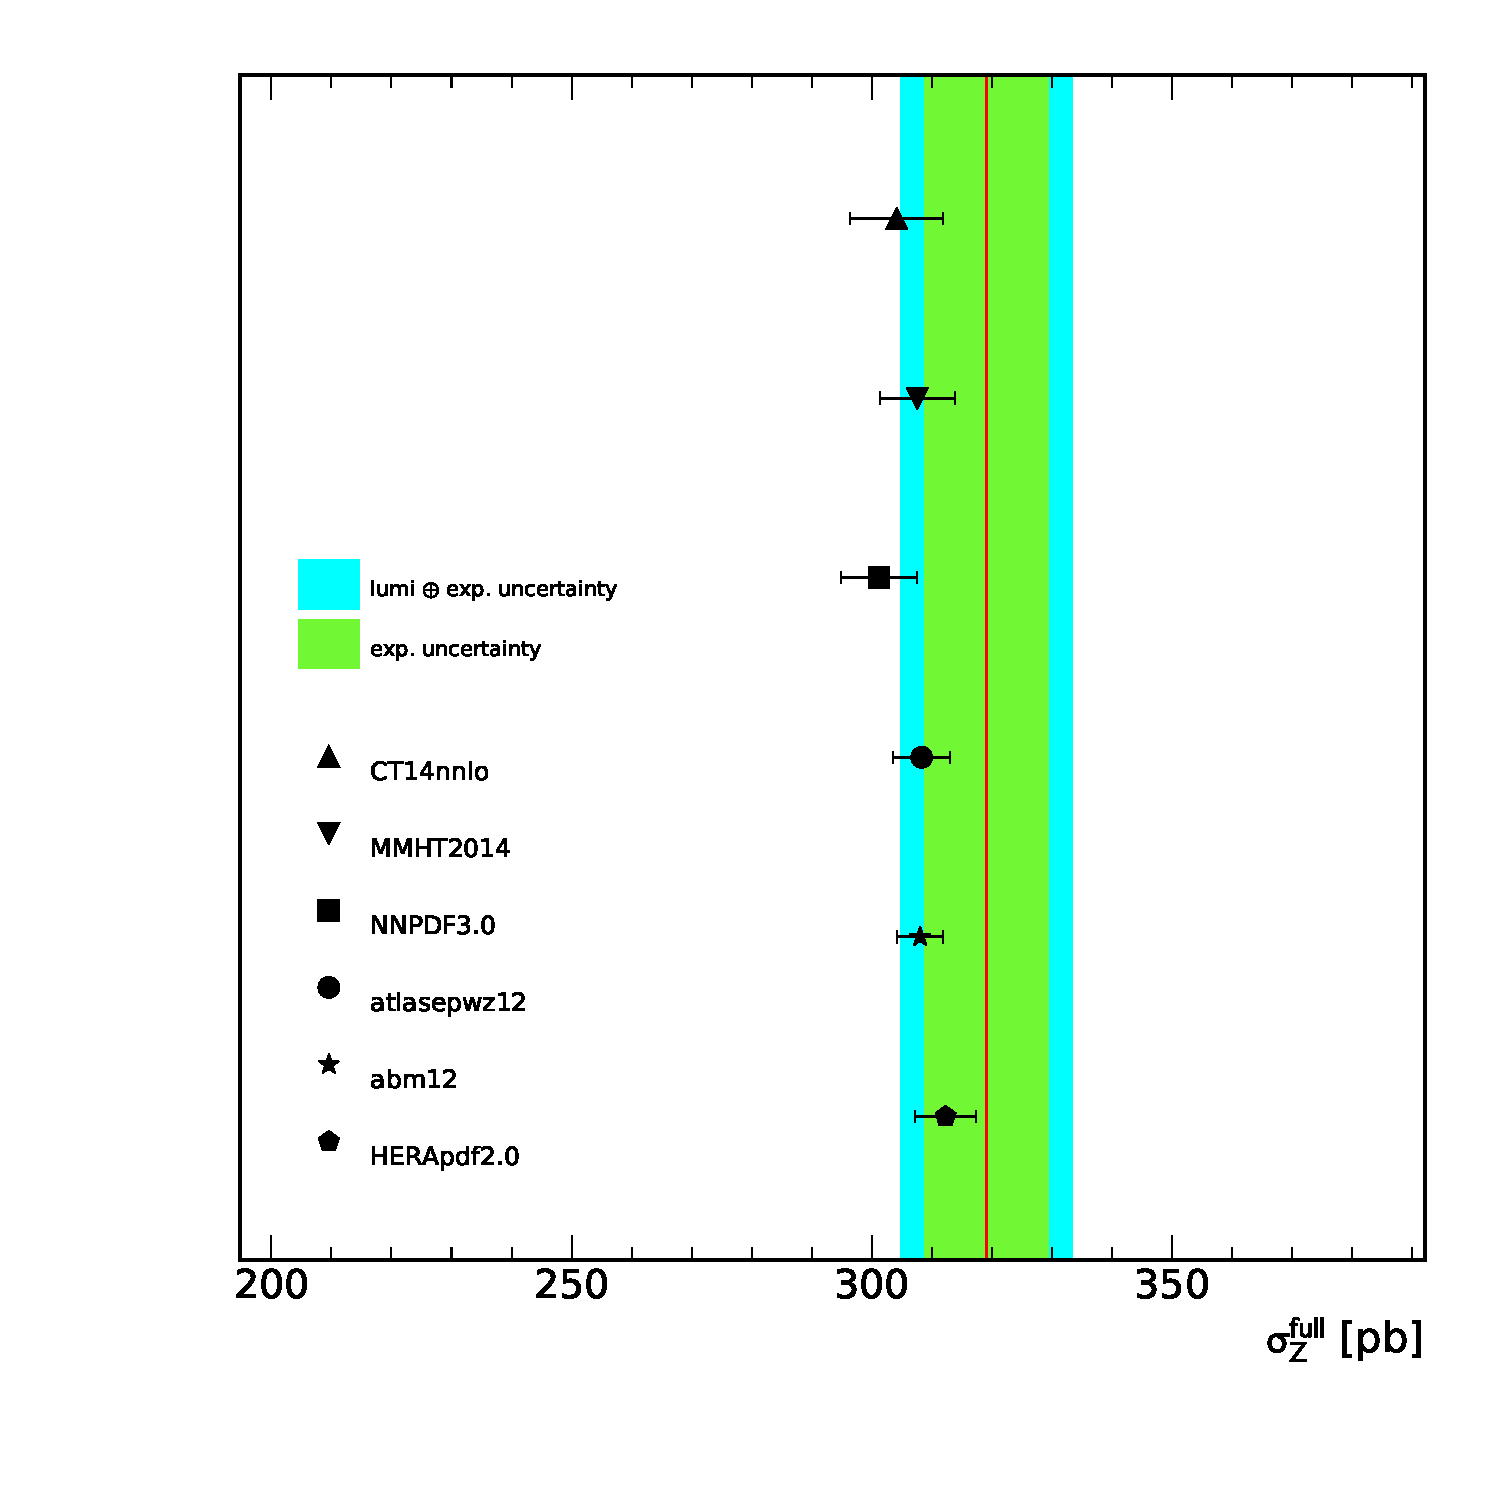
\includegraphics[width=1.0\textwidth]{Results/NNLOZfull.pdf} \\ a)}
\end{minipage}
\hfill
\begin{minipage}[h]{0.49\linewidth}
\center{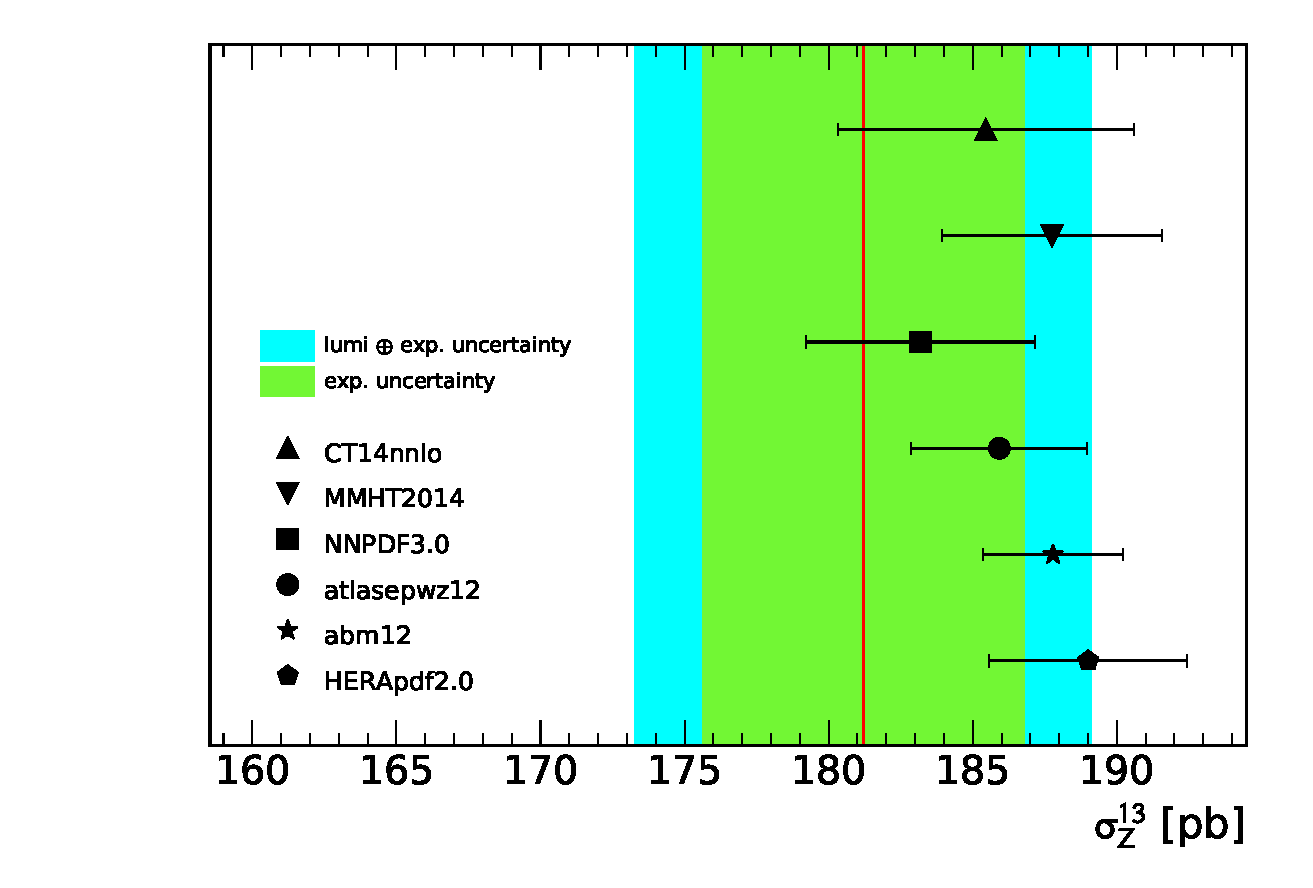
\includegraphics[width=1.0\textwidth]{Results/NNLOZ13.pdf} \\ b)}
\end{minipage}
\caption{The NNLO predictions for the $Z$ cross section in a) full phase space and  b) new 13 TeV phase space in pb for the six PDFs CT14nnlo, MMHT2014, NNPDF3.0, ATLASepWZ12, abm12, HERApdf2.0 compared to the measured cross section as given in Tab.~\ref{tab:csComb}. The green (cyan) band corresponds to the experimental uncertainty without (with) the luminosity uncertainty. The theory predictions are given with the corresponding PDF uncertainties shown as error bands.}
\label{fig:AppD3}
\end{figure}

\begin{figure}[!h]
\begin{minipage}[h]{0.45\linewidth}
\center{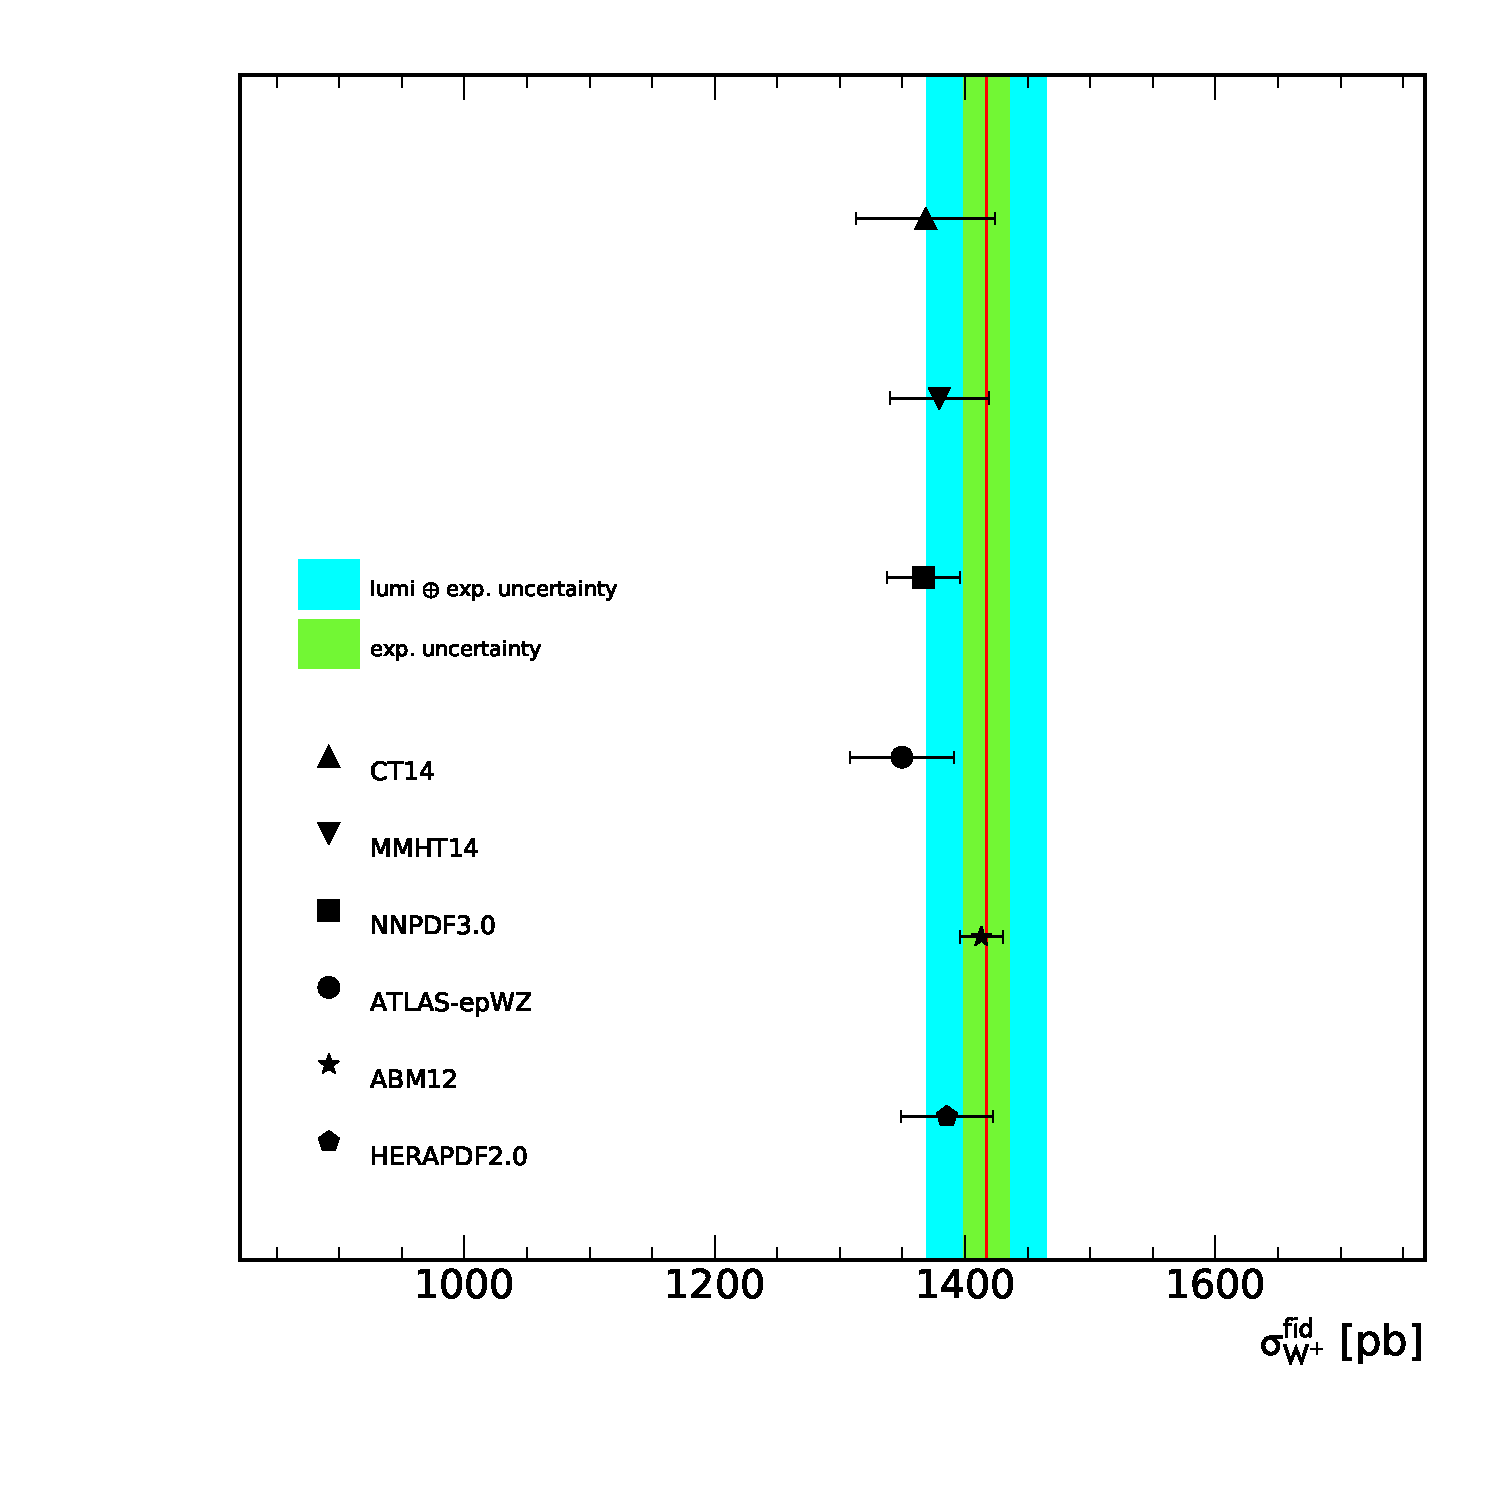
\includegraphics[width=1\textwidth]{Results/NLOWp.pdf} \\ a)}
\end{minipage}
\hfill
\begin{minipage}[h]{0.45\linewidth}
\center{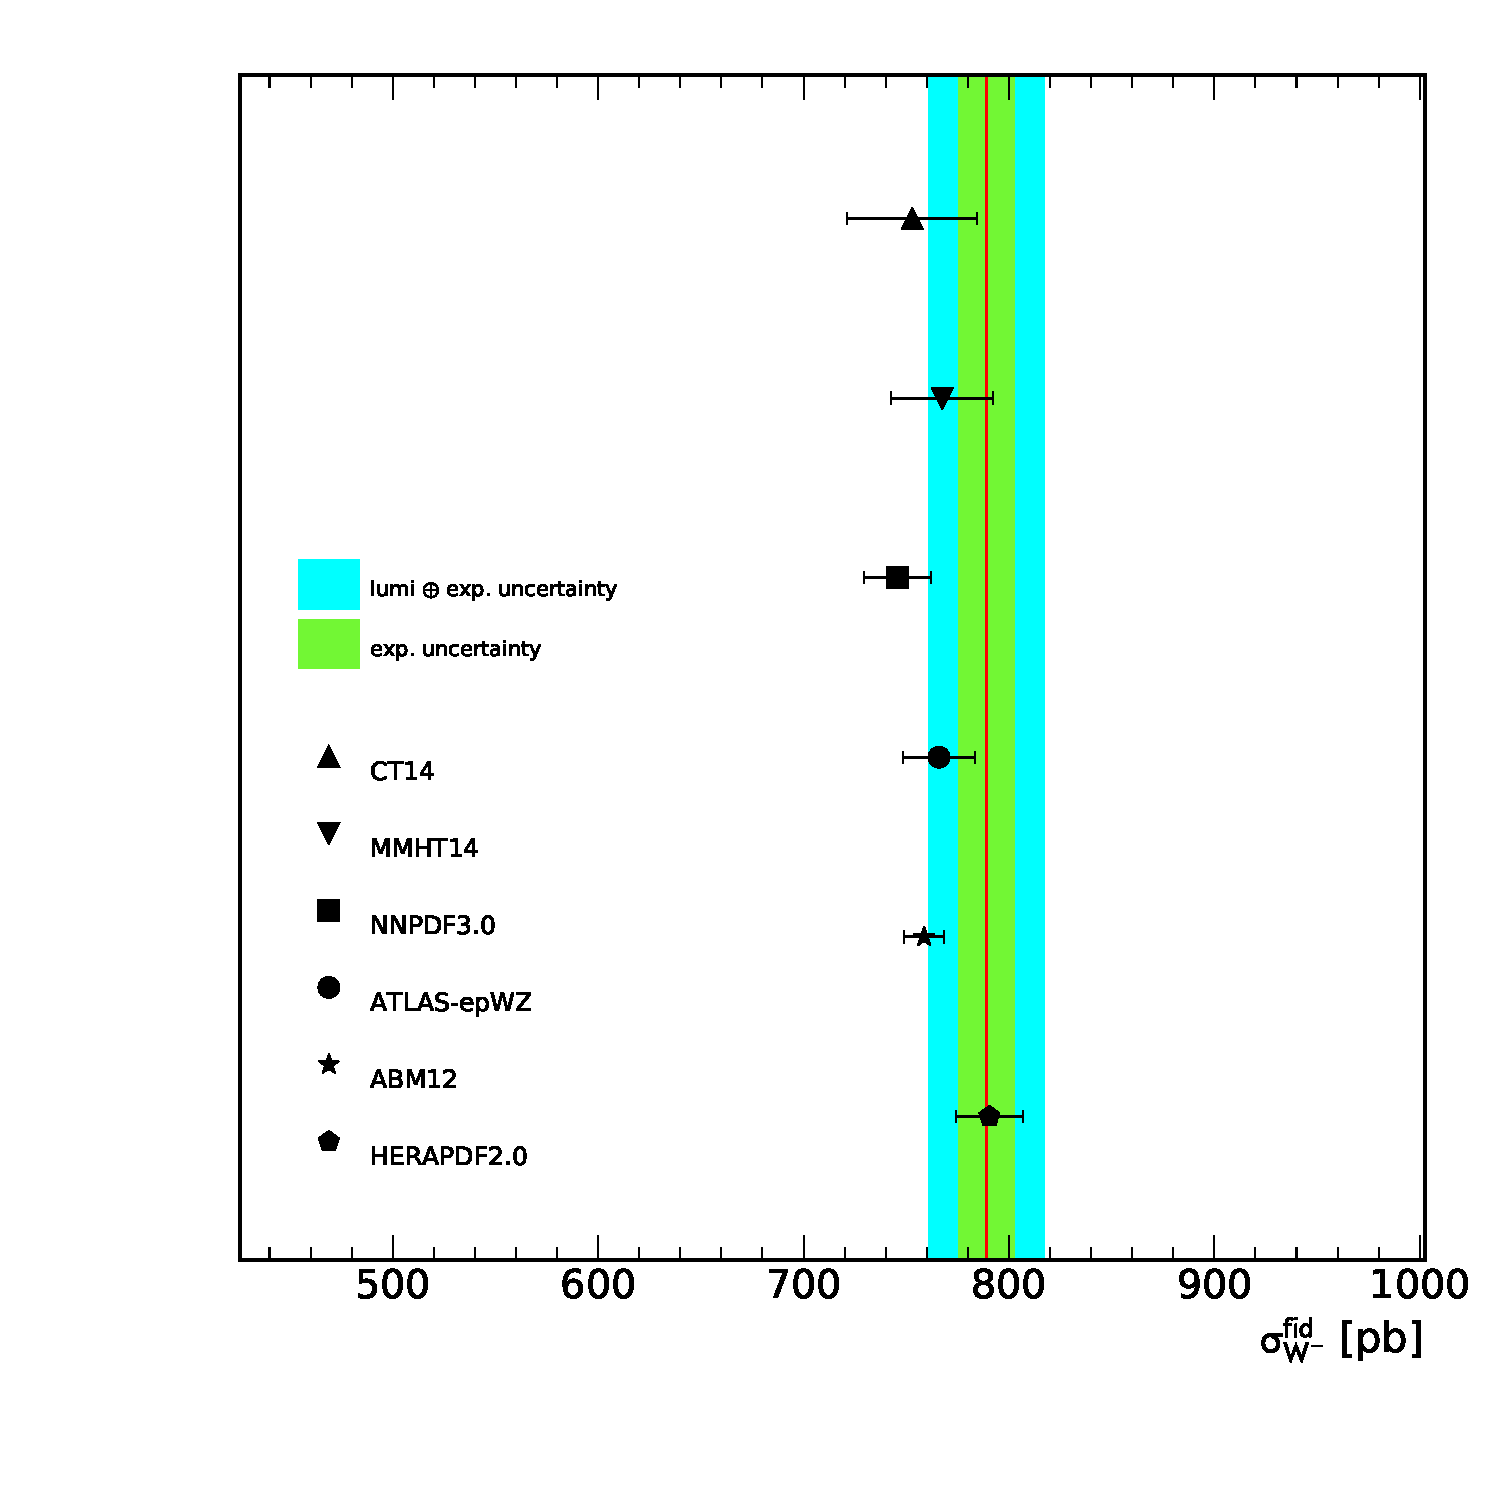
\includegraphics[width=1\textwidth]{Results/NLOWm.pdf} \\ b)}
\end{minipage}
\caption{The NLO predictions for the fiducial cross section a) $\sigma^{fid}_{W^+}$  b) $\sigma^{fid}_{W^-}$  in pb for the six PDFs CT14nnlo, MMHT2014, NNPDF3.0, ATLASepWZ12, abm12, HERApdf2.0 compared to the measured fiducial cross section as given in Tab.~\ref{tab:csComb}. The green (cyan) band corresponds to the experimental uncertainty without (with) the luminosity uncertainty. The theory predictions are given with the corresponding PDF uncertainties shown as error bands.}
\label{fig:AppD4}
\end{figure}

\begin{figure}[!h]
\center{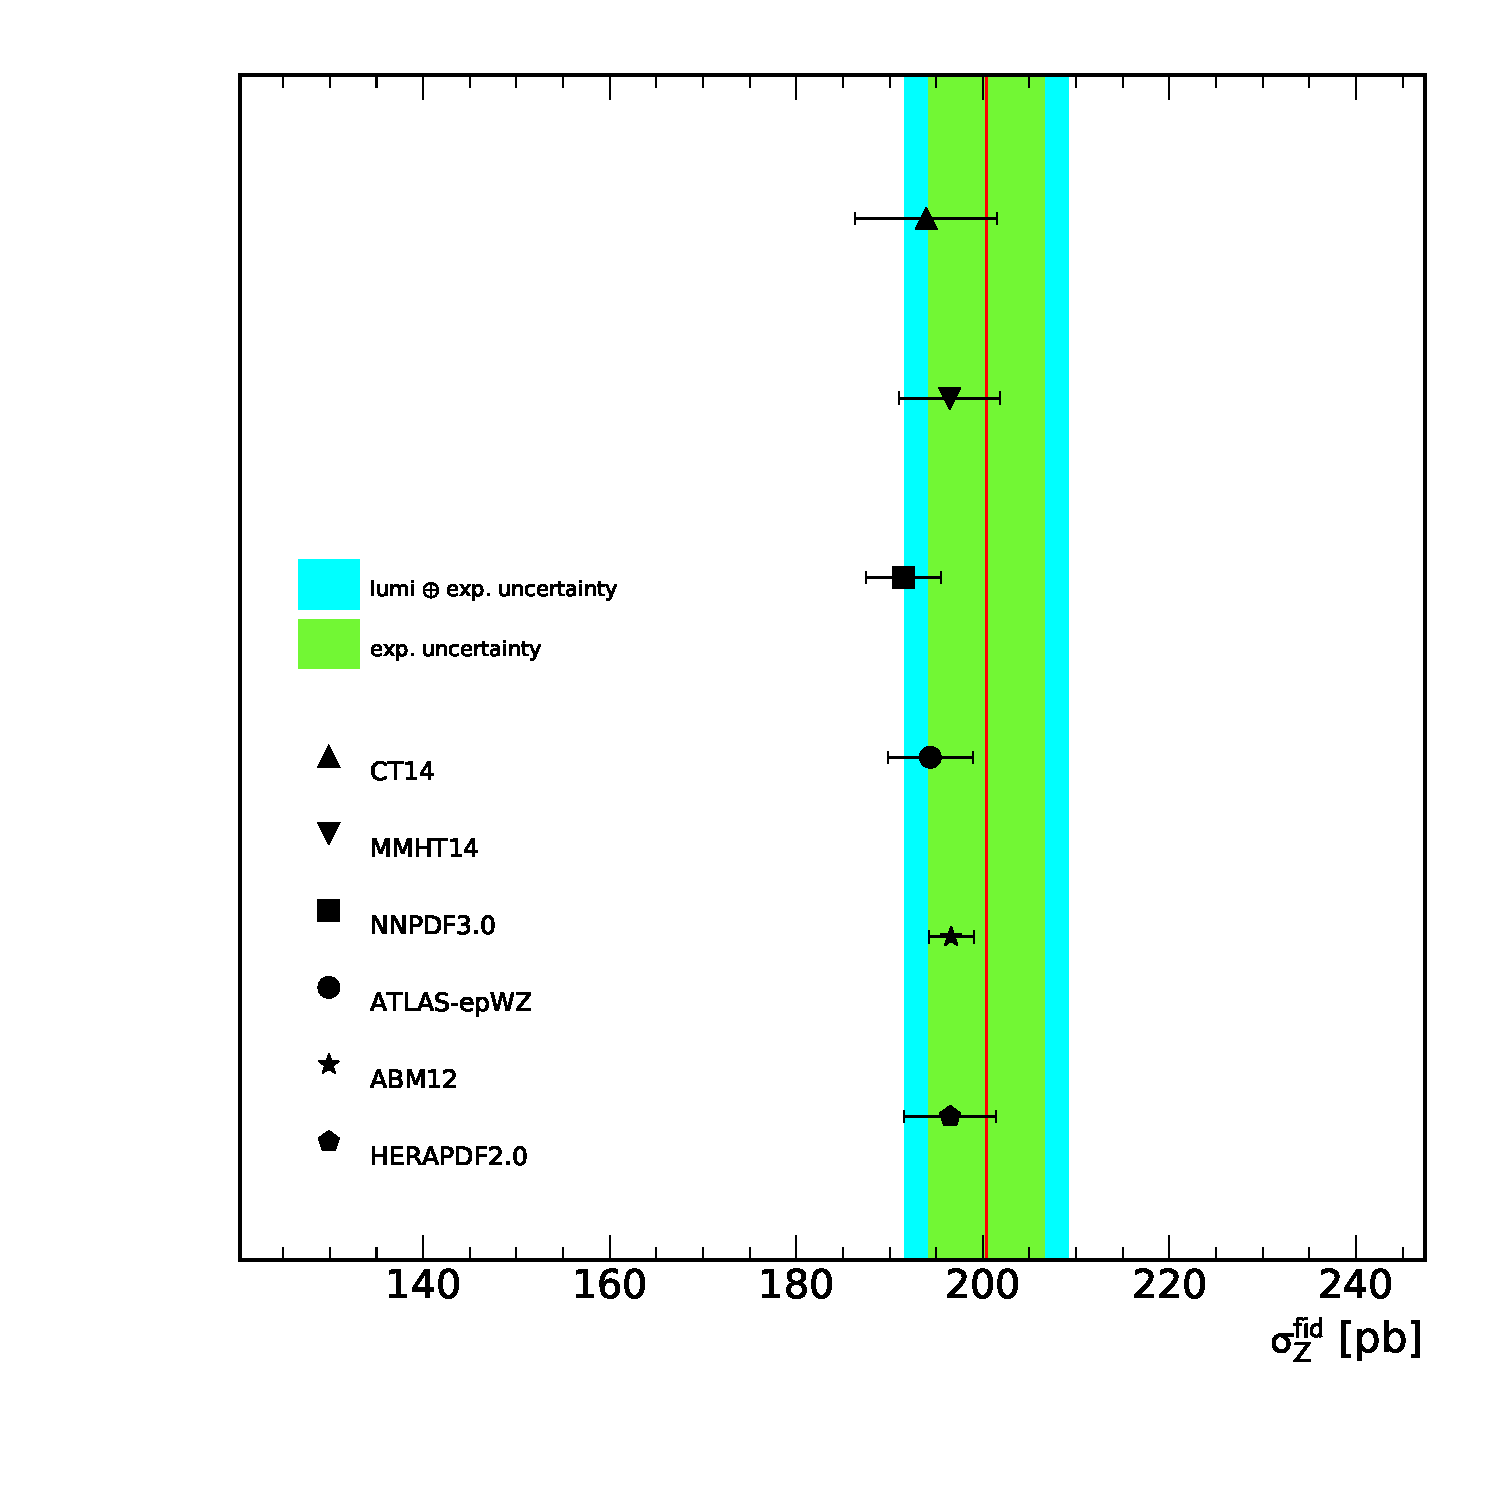
\includegraphics[width=0.45\textwidth]{Results/NLOZ.pdf}}
\caption{The NLO predictions for the fiducial cross section $\sigma^{fid}_Z$ in pb for the six PDFs CT14nnlo, MMHT2014, NNPDF3.0, ATLASepWZ12, abm12, HERApdf2.0 compared to the measured fiducial cross section as given in Tab.~\ref{tab:csComb}. The green (cyan) band corresponds to the experimental uncertainty without (with) the luminosity uncertainty. The theory predictions are given with the corresponding PDF uncertainties shown as error bands.}
\label{fig:AppD5}
\end{figure}


\chapter{Additional PDF profiling plots}\label{app:PDF}

The results of PDF profiling have been showed in Sec.~\ref{sec:PDFCs}. In this Appendix the effect on valence quarks ratio $d_{v}/u_{v}$ (Fig.~\ref{fig:AppC1}) and difference in sea u and d quarks $\bar{d}-\bar{u}$ (Fig.~\ref{fig:AppC2}) is shown. The effect of inclusion of the new data at the scale of the measurement $Q^2 \approx M^2_{W}$ is shown in Fig.~\ref{fig:AppC3}-~\ref{fig:AppC4}. 

\begin{figure}[!h]
\begin{minipage}[h]{0.49\linewidth}
\center{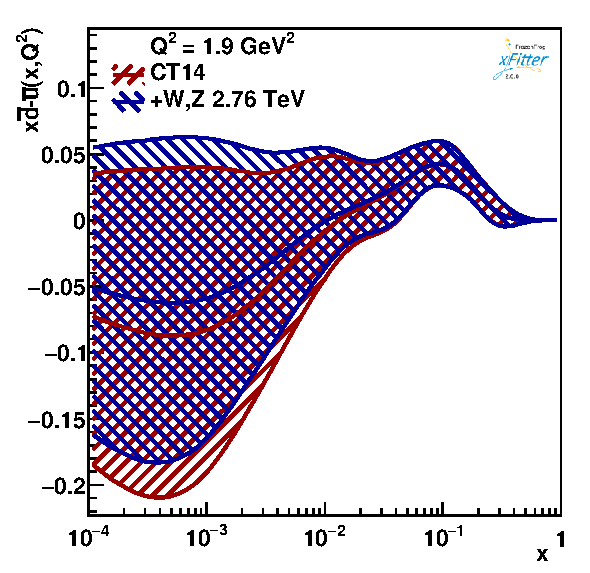
\includegraphics[width=1\textwidth]{Results/Shift/dbar-ubar.pdf} \\ a)}
\end{minipage}
\hfill
\begin{minipage}[h]{0.49\linewidth}
\center{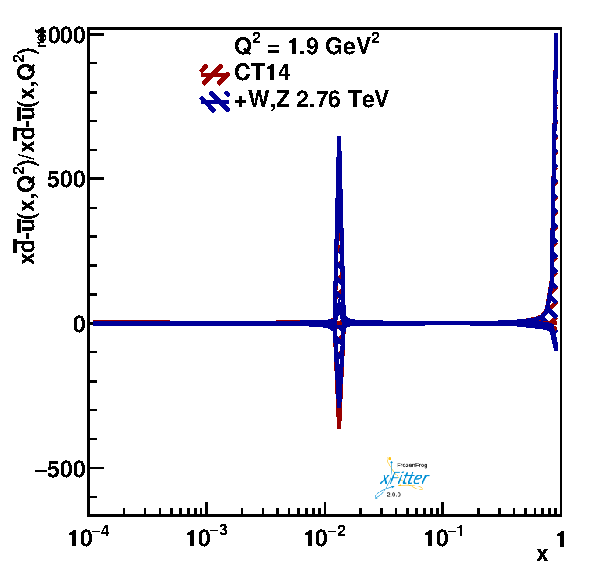
\includegraphics[width=1\textwidth]{Results/Shift/dbar-ubar_ratio.pdf} \\ b)}
\end{minipage}
\caption{The a) absolute and  b) relative distributions for the $\bar{d}-\bar{u}$ quark densities as a function of $x$ at scale $Q^2=$ 1.9 GeV$^2$ with the experimental uncertainties. The red band denotes the reference NLO PDF distributions from CT14 pdf set. The impact of addition of the new W,Z cross sections at 2.76 TeV on the PDF set is shown by the blue boundaries.}
\label{fig:AppC1}
\end{figure}

\begin{figure}[!h]
\begin{minipage}[h]{0.49\linewidth}
\center{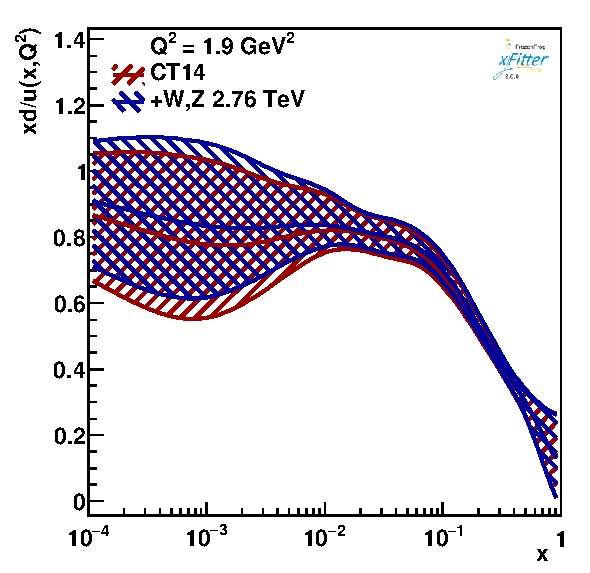
\includegraphics[width=1\textwidth]{Results/Shift/doveru.pdf} \\ a)}
\end{minipage}
\hfill
\begin{minipage}[h]{0.49\linewidth}
\center{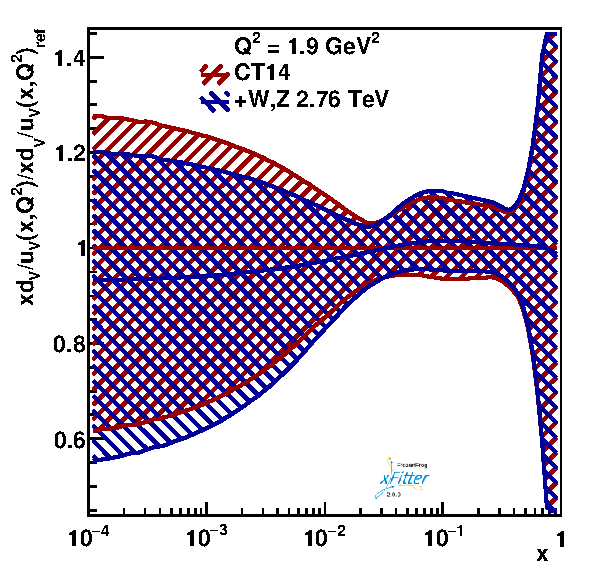
\includegraphics[width=1\textwidth]{Results/Shift/dvoveruv_ratio.pdf} \\ b)}
\end{minipage}
\caption{The a) absolute and  b) relative distributions for the $u_v / d_v$ quark densities as a function of $x$ at scale $Q^2=$ 1.9 GeV$^2$ with the experimental uncertainties. The red band denotes the reference NLO PDF distributions from CT14 pdf set. The impact of addition of the new W,Z cross sections at 2.76 TeV on the PDF set is shown by the blue boundaries}
\label{fig:AppC2}
\end{figure}

\begin{figure}[!h]
\begin{minipage}[h]{0.49\linewidth}
\center{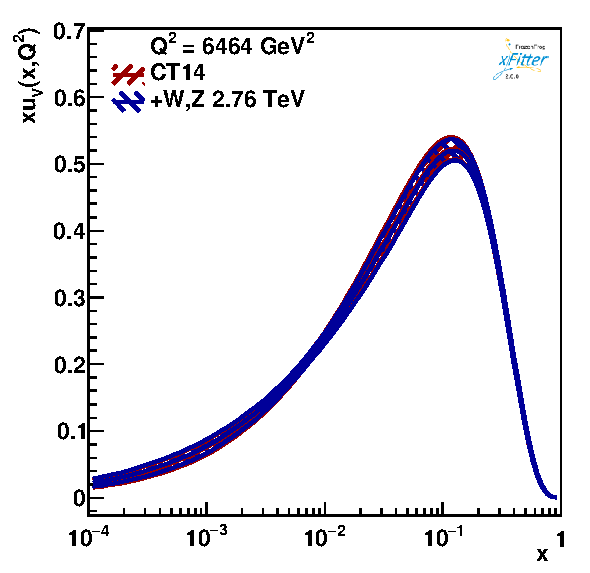
\includegraphics[width=1\textwidth]{Results/Q2Evol/q2_6464_pdf_uv.pdf} \\ a)}
\end{minipage}
\hfill
\begin{minipage}[h]{0.49\linewidth}
\center{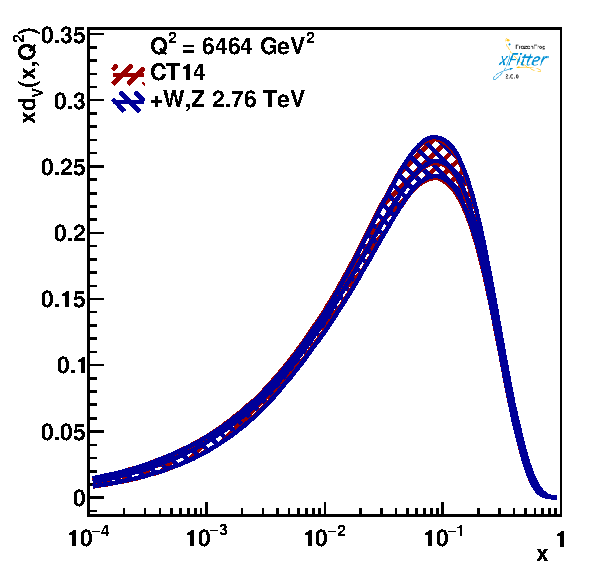
\includegraphics[width=1\textwidth]{Results/Q2Evol/q2_6464_pdf_dv.pdf} \\ b)}
\end{minipage}
\caption{The absolute for the a) $u_v$ and b) $d_v$ quark densities as a function of $x$ at scale $Q^2=M_W^2$ with the experimental uncertainties. The red band denotes the reference NLO PDF distributions from CT14 pdf set. The impact of addition of the new W,Z cross sections at 2.76 TeV on the PDF set is shown by the blue boundaries.}
\label{fig:AppC3}
\end{figure}

\begin{figure}[!h]
\begin{minipage}[h]{0.49\linewidth}
\center{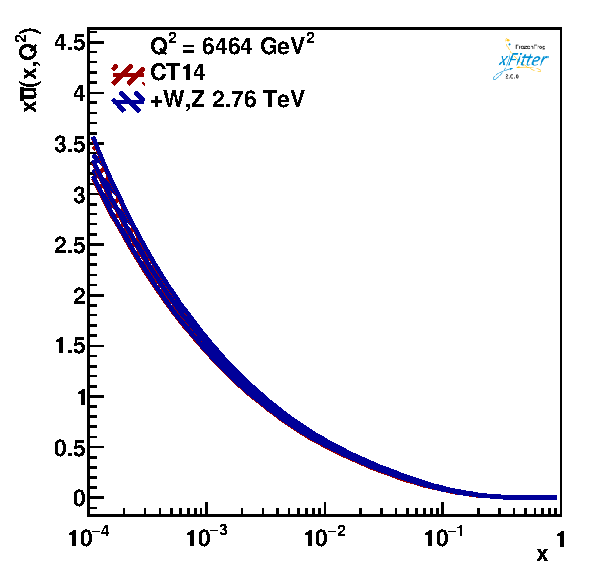
\includegraphics[width=1\textwidth]{Results/Q2Evol/q2_6464_pdf_UBar.pdf} \\ c)}
\end{minipage}
\hfill
\begin{minipage}[h]{0.49\linewidth}
\center{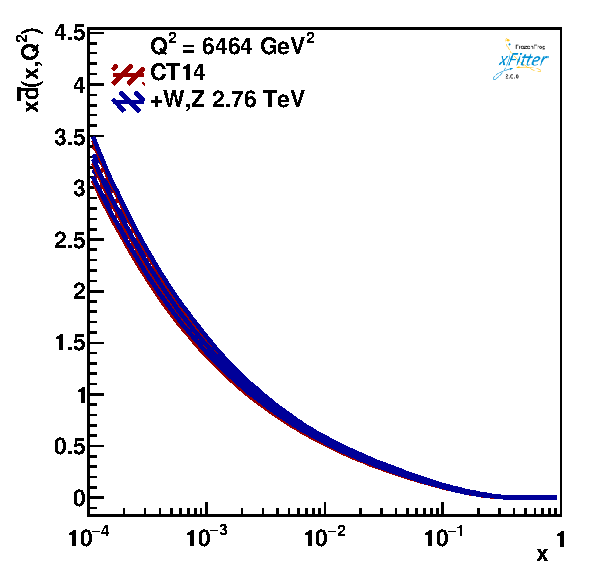
\includegraphics[width=1\textwidth]{Results/Q2Evol/q2_6464_pdf_DBar.pdf} \\ d)}
\end{minipage}
\caption{The absolute for the a) $\bar{u}$ and b) $\bar{d}$ quark densities as a function of $x$ at scale $Q^2=M_W^2$ with the experimental uncertainties. The red band denotes the reference NLO PDF distributions from CT14 pdf set. The impact of addition of the new W,Z cross sections at 2.76 TeV on the PDF set is shown by the blue boundaries.}
\end{figure}

\begin{figure}[!h]
\begin{minipage}[h]{0.49\linewidth}
\center{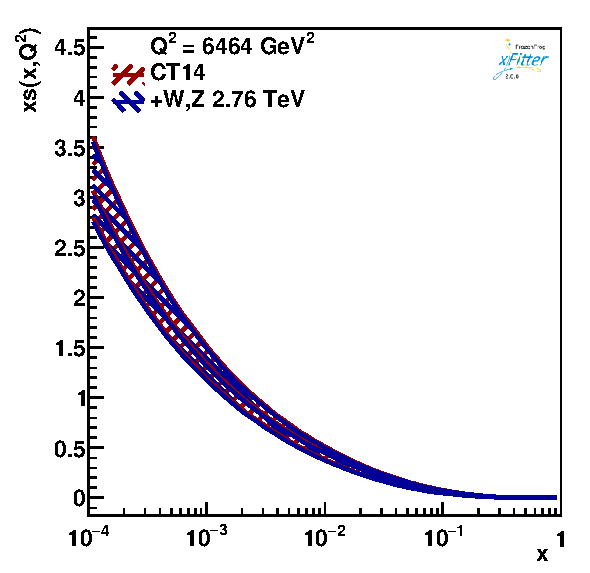
\includegraphics[width=1\textwidth]{Results/Q2Evol/q2_6464_pdf_s.pdf} \\ e)}
\end{minipage}
\hfill
\begin{minipage}[h]{0.49\linewidth}
\center{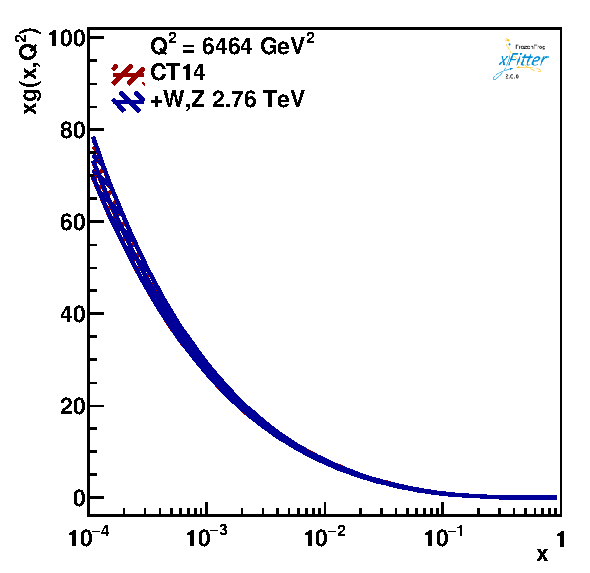
\includegraphics[width=1\textwidth]{Results/Q2Evol/q2_6464_pdf_g.pdf} \\ f)}
\end{minipage}
\caption{The absolute for the a) $s$ quark and b) gluon densities as a function of $x$ at scale $Q^2=M_W^2$ with the experimental uncertainties. The red band denotes the reference NLO PDF distributions from CT14 pdf set. The impact of addition of the new W,Z cross sections at 2.76 TeV on the PDF set is shown by the blue boundaries.}
\label{fig:AppC4}
\end{figure}
